\documentclass[
	papersize=A4,
		%% e.g., "A4", "letter", "legal", "executive", ...
		%% The size of the paper of the resulting PDF file.	
	fontsize=12pt, 
	 	%% e.g., 10pt, 11pt, 12pt
	 	%% The font size of the main text in pt (points).
	laterality=oneside, 
	 	%% "oneside" or "twoside"
	 	%% Either you are creating a document which is printed on both, left pages
	 	%% and right pages (twoside) or you create a document which is printed
	 	%% on right pages only (oneside).
	draft=false,
	 	%% "true" or "false"
	 	%% Use draft mode? If true, included graphics are replaced by empty
	 	%% rectangles (of same size) and overfull boxes (in margin space) are
	 	%% marked with black box (-> easy to spot!)
	parskip=half,
	 	%% e.g., "no", "full", "half", ...
	 	%% How to separate paragraphs: indention ("no") or spacing ("half",
	 	%% "full", ...).
	BCOR=0mm,
	 	%% Inner binding correction. This value depends on the method which is
	 	%% being used to bind your printed result. Some techniques do not
	 	%% require a binding correction at all ("0mm"), other require for
	 	%% example "5mm". Refer to KOMA script documentation for a detailed
	 	%% explanation what a binding correction is and how to measure it.
	linespread=1.15,
	 	%% e.g., 1.0, 1.5, 2.0
	 	%% Line spacing in %/100. For example 1.5 means 150% of the usual line
	 	%% spacing. Please use with caution: 100% ("1.0") is fine because the
	 	%% font was designed for it.
	language={english,ngerman},
	 	%% "english,ngerman", "ngerman,english", ...
	 	%% NOTE: The *last* language is the active one!
	 	%% See babel documentation for further details.
	biblatex, % use biblatex
	% bibtex % use bibtex
		%% Choose the bibliography system you want to use, either 
		%% "biblatex" or "bibtex". Note that you also have to change the 
		%% bibfile below to reflect the correct one. 
	bibfile=99--references.bib,
	% bibfile=references-bibtex.bib,
	 	%% Name of the biblatex file that holds the references.
	biblatexstyle=alphabetic,
	% biblatexstyle=authoryear,
	 	%% BibLaTeX-settings: (see biblatex reference for further description)
	 	%% e.g., "alphabetic", "authoryear", ...
	 	%% The biblatex style which is being used for referencing. See
	 	%% biblatex documentation for further details and more values.
	 	%%
	 	%% CAUTION: if you change the style, please check for (in)compatible
	 	%%          "biblatex" package options in the file
	 	%%          "template/preamble.tex"! For example: "alphabetic" does
	 	%%          not have an option "dashed=..." and causes an error if it
	 	%%          does not get removed from the list of options.
	biblatexdashed=false,  %% "true" or "false"
	 	%% If true: replace recurring reference authors with a dash.
	biblatexbackref=true,  %% "true" or "false"
	 	%% If true: create backward links from reference to citations.
	bibtexstyle=alpha, 
		%% bibtex style to use, e.g. "alpha", "plain", "authordate1", ...
	dispositioncolor={30,103,182},
        % dispositioncolor={0.9636,0.5287,0,0},
	 	%% e.g., "30,103,182" (blue/turquois), "0,0,0" (black), ...
	 	%% Color of the headings and so forth in RGB (red,green,blue) values.
	colorlinks=true, %% "true" or "false"
	 	%% Enables or disables colored links (hyperref package).
    titlepage=titlepage,
	 	%% file name (without .tex) of title page file in template/ directory
	todonotesoptions={color=Dandelion,bordercolor=white},
	 	%% e.g., "" (empty), "disable", ...
	 	%% Options for the todonotes-package. If "disable", all todonotes will
	 	%% be hidden (including listoftodos).
	addcolophon=false, %% "true" or "false"
		%% If set to "true": a colophon (with notes about this document
		%% template, LaTeX, ...) is added after the title page.
		%% Please do not set to "false" without a good reason. The colophon
		%% helps your readers to get in touch with LaTeX and to find this template.
	addlistoftodos=false, %% "true" or "false"
		%% If set to "true": the current list of open todos is added after the
		%% table of contents. If \mytodonotesoptions is set to "disable", no
		%% list of todos is added, independent of this setting here.
]{longdoc}

% \addbibresource{99--references.bib} % for sublime text completion to work

%% ========================================================================
%%%% Document metadata
%% ========================================================================

%% general metadata:
\LDauthor{Max Mustermann} 
\LDtitle{Entwurf eines Versuchsstandes für Kreiselpumpen}
\LDsubject{Subject used for PDF Info}  
\LDkeywords{Keywords used for PDF Info} 

%% this information is used only for generating the title page:
\LDworktitle{DIPLOMARBEIT}  
\LDuniversity{Technische Universität Humbug} 
\LDinstitute{Institut für Dokumentenerstellung}
\LDinstitutehead{Univ.-Prof.\ Dipl.-Ing.\ Dr.\,techn.~Hans Wurst} 
\LDsupervisor{Univ.-Prof.\ Dipl.-Ing.\ Dr.\,techn.~Franz Fraß} 
\LDcosupervisor{Dipl.-Ing.\ Dr.\,techn.~Max Mann}
\LDevaluator{Univ.-Prof.\ Dipl.-Ing.\ Dr.techn.~Ingo Igel} 
% \LDhomestreet{} %% your home street (with house number)
\LDhometown{Humbug} %% your home town
\LDhomepostalnumber{1234} %% your postal number of home town
\LDsubmissionmonth{Juli} %% month you are handing in
\LDsubmissionyear{2045} %% year you are handing in
\LDsubmissiontown{\LDinserthometown} %% town of handing in (or \myhometown)

%% additional information for generic_documentation title page
% \LDid{1234567} %% Matrikelnummer
% \LDlecture{LECTURE} %% 

% \usepackage{showframe} % shows the text frame (margins)

\newcommand{\centeredsection}[1]{{\let\raggedsection\centering\section*{#1}}}
\newcommand{\zB}{z.\,B.\xspace}
\newcommand{\usw}{usw.\xspace}
\newcommand{\etc}{etc.\xspace}
\newcommand{\bzw}{bzw.\xspace}
\renewcommand{\dh}{d.\,h.\xspace}


%% ========================================================================
%%%% Main Document
%% ========================================================================

\begin{document}

% siehe https://docs.google.com/document/d/1aJE58I_N8w1tfuHNkwBzOSTkf6Wr4mj7EjtUQLPJhS0/edit#

\chapter{Einleitung}

Kurzbeschreibung des Gesamtthemas: Wie lautet das Thema? Welche Hintergründe gibt es (wie sieht das fachliche bzw. wirtschaftliche Umfeld aus)? Was ist darüber bekannt?

Beschreibung der Leistung: Was ist das Ziel des Gesamtprojektes? Für wen hat die Arbeit Relevanz? Wer sind die Kooperationspartner? Welche Methoden werden angewendet? Welches Produkt soll erstellt werden? Welche Daten werden dafür gesammelt?

Welche Abgrenzung gibt es zu den eigenen SYP-Projekten der vierten und fünften Klasse.

Darstellung der Vorgehensweise: Welches Vorgehensmodell wurde gewählt (inkl. Begründung der Entscheidung für dieses Vorgehensmodell => Quellen!!)? In welche Kapitel ist die Arbeit gegliedert? Was steht in diesen Kapiteln?

Zeit: Gegenwart

\chapter{Kooperationsvereinbarung}

zwischen 

1. \emph{Name des Kooperationspartners/Unternehmens} vertreten durch Name der Vertreterin/des Vertreters – in der Folge "`die Projektpartnerin/der Projektpartner"' 

und 

2. \emph{Name der Schüler/innen} – in der Folge "`das Projektteam"'

\centeredsection{Präambel}

Das Projektteam und die Projektpartnerin/der Projektpartner beabsichtigen gemäß der Verordnung über die abschließenden Prüfungen in den berufsbildenden mittleren und höheren Schulen, BGB. II Nr. 70/2000 vom 24.2.2000, die Planung und Durchführung eines Diplomprojekts, welches die Erstellung eines Konzeptes einer kostenoptimierten Instandhaltung als Ziel hat. Durch die Zusammenarbeit soll insbesondere den Mitgliedern des Projektteams die Möglichkeit eingeräumt werden, im Rahmen ihrer schulischen Ausbildung bei der Erstellung der Diplomarbeit an die Verhältnisse im technischen Berufsleben herangeführt zu werden, um dabei die in der Schule erworbenen theoretischen Kenntnisse und Fähigkeiten in der Praxis anzuwenden bzw. zu erweitern. Hingewiesen wird in diesem Zusammenhang auf den unentgeltlichen Charakter dieser Vereinbarung. 

\centeredsection{§ 1 Gegenstand}
Gegenstand ist die Erstellung von Arbeitsergebnissen zum Thema der Diplomarbeit. Dieses Thema ist der Projektbeschreibung und dem Pflichtenheft zu entnehmen, welches der Kooperationsvereinbarung beiliegt. Die Projektpartnerin/Der Projektpartner wird jedoch darauf hingewiesen, dass es sich um ein Projekt im Zusammenhang mit der schulischen Ausbildung handelt und daher jede Haftung des Projektteams, insbesondere in Hinsicht auf die Unentgeltlichkeit des Vertrages, ausgeschlossen ist. Nutzungs- und Verwertungsrechte von im Rahmen dieser Vereinbarung erstellten Arbeitsergebnissen stehen der Projektpartnerin/dem Projektpartner sowie dem Projektteam gemeinsam zu. 

\centeredsection{§ 2 Laufzeit}
Die vorliegende Kooperation tritt am \emph{\color{red}Datum einsetzen} in Kraft und wird bis zum Ende der Reife- und Diplomprüfung der HTL Pinkafeld abgeschlossen. 

\centeredsection{§ 3 Rechte und Pflichten des Projektteams}
Die Mitglieder des Projektteams haben das Recht, die Räumlichkeiten der Projektpartnerin/des Projektpartners samt Infrastruktur und EDV-Infrastruktur im für die Projektabwicklung erforderlichen Ausmaß nach vorheriger schriftlicher Genehmigung durch die Projektpartnerin/den Projektpartner mitzubenutzen. Das Projektteam verpflichtet sich, die im Gegenstand genannten Arbeiten sorgfältig und unter möglichster Schonung der Interessen der Projektpartnerin/des Projektpartners durchzuführen. Das Projektteam unterliegt der Betriebsordnung der Projektpartnerin/des Projektpartners. Das Projektteam verpflichtet sich zur Geheimhaltung aller ihm zur Kenntnis gelangenden Geschäfts- und Betriebsgeheimnisse. 

\centeredsection{§ 4 Rechte und Pflichten der Projektpartnerin/des Projektpartners}
Die Projektpartnerin/Der Projektpartner verpflichtet sich, dem Projektteam beratend zur Verfügung zu stehen und alles zu unterlassen, was der Vollendung des Projekts entgegensteht. Die Projektpartnerin/Der Projektpartner verpflichtet sich, dem Projektteam folgende Hilfsmittel zur Verfügung zu stellen: 
\begin{itemize}
    \item ...
    \item ...
\end{itemize}

Sollte das Projektteam im Rahmen dieser Kooperationsvereinbarung eine Erfindung machen, die nach dem Gebrauchsmustergesetz bzw. dem Patentgesetz (PatG) schützbar ist, gilt diese Erfindung als Diensterfindung im Sinne des PatG und die §§ 6-19 PatG (in der geltenden Fassung) entsprechend. Das Projektteam verpflichtet sich, die Projektpartnerin/den Projektpartner von einer im Rahmen der Kooperationsvereinbarung gemachten Erfindung unverzüglich in Kenntnis zu setzen. Die Projektpartnerin/Der Projektpartner hat daraufhin das Recht, binnen vier Wochen ab dieser Bekanntgabe zu erklären, dass sie/er das Patentrecht für dich beansprucht. In diesem Fall steht dem Projektteam eine entsprechende Vergütung nach den einschlägigen Bestimmungen des PatG (in der geltenden Fassung) zu. Sollte das Projektteam im Rahmen dieser Kooperationsvereinbarung ein Werk schaffen, dem Schutz im Sinne des Urheberrechtsgesetzes zukommt, verpflichtet es sich, die Projektpartnerin/den Projektpartner davon unverzüglich zu informieren. Die Projektpartnerin/Der Projektpartner hat daraufhin die Möglichkeit, binnen vier Wochen ab dieser Bekanntgabe, mit dem Projektteam einen Werknutzungsvertrag abzuschließen. 

\centeredsection{§ 5 Einsicht und Präsentation}
Da die Tätigkeit des Projektteams auch Inhalt bzw. Grundlage der an der HTL Pinkafeld zu erstellenden Diplomarbeit ist, berechtigt die Projektpartnerin/der Projektpartner die zuständigen Organe des Bundes zur Einsicht und Kontrolle, um die in der Verordnung über die abschließenden Prüfungen an den berufsbildenden höheren Schulen genannten Aufgaben zu erfüllen. Das Projektteam ist auch berechtigt, Ergebnisse der Diplomarbeit bei der mündlichen Reife- und Diplomprüfung zu präsentieren. Die zuständigen Organe des Bundes sind ihrerseits wiederum gegenüber jedermann zur Geschäfts- und Betriebsgeheimnisse der Projektpartnerin/des Projektpartners verpflichtet. 

\vspace*{1cm}

\hspace*{\fill}\begin{tabular}{cp{2em}c} 
   \hspace{4cm}        & & \hspace{6cm} \\\cline{1-1}\cline{3-3}
                       & & \\[-3mm]
   {\footnotesize Ort, Datum }  & & {\footnotesize Projektpartner/in }
\end{tabular}\hspace*{\fill}

\vspace*{1cm}

\hspace*{\fill}\begin{tabular}{cp{2em}c} 
   \hspace{4cm}        & & \hspace{6cm} \\\cline{1-1}\cline{3-3}
                       & & \\[-3mm]
   {\footnotesize Ort, Datum }  & & {\footnotesize Projektteam }
\end{tabular}\hspace*{\fill}

\chapter{Projektantrag}

gemäß DA-Datenbank


\chapter{Projektvorstudie}

\begin{itemize}
\item Istsituation (Description of actual condition, Use cases, activity diagrams)
\item Stärken-, Schwächen Analyse (Strength-, Weaknesses analysis), evtl. SWOT
\item Generelle Ziele und (davon abgeleitete) konkrete (messbare) Zielsetzung und Ergebnisse (Goals, objectives and deliverables)
\item Grobe Anforderungen (Requirements on a higher level)
\item Alternative Lösungen (Alternative solutions)
\item Entscheidungsfindung (Decision for a solution, Value-benefit analysis)
\item Evtl Machbarkeitsstudie (feasibility study)
\item Grobschätzung (Rough estimation, Work breakdown structure (WBS))
\item Kosten-Nutzen Analyse (Cost-benefit analysis)
\item Achtung: Wenn Teile der Vorstudie einen speziellen Bezug zu einer der individuellen Themenstellung eines der Diplomanden haben, dann sind diese in dessen individuellen Teil anzuführen. (Beispiel: Schüler A hat die Themenstellung “...unter Berücksichtigung der Barrierefreiheit”, dann sind diese Analysen in dessen Teil anzuführen!)

\end{itemize}

\chapter{Individueller Teil Schüler 1}

Vordergründig sollte der individuelle Teil enthalten:
\begin{itemize}
    \item Evaluierung von Technologien und/oder Frameworks
    \item Beschreibung von Lösungsansätzen mit Vor- und Nachteilen
    \item Beschreibung von technischen aber auch organisatorischen Problemen und Lösungsansätze
\end{itemize}

Bestandteile können unter anderem sein:
\begin{itemize}
    \item Designentwurf (Mockups: nicht alle Mockups, sondern nur der prinzipielle Aufbau der Bildschirmmasken, eventuell: je ein Beispiel für eine Listanzeige und eine Einzelbearbeitung)
    \item Projektplanung
        \begin{itemize}
            \item Aufwandschätzung
            \item Gantt-Chart
            \item Meilensteinplan
            \item Risikoanalyse
            \item Projektumwelt(en)
            \item Stakeholderanalyse
            \item Produktbacklog, Sprint-Backlog
            \item Beispiel Sprintplanung
            \item Projekt-Retrospektive
        \end{itemize}
    \item technische Realisierung
        \begin{itemize}
            \item Das techn. System im Hintergrund (Systemarchitektur, ..)
            \item Klassendiagramm
            \item Paketdiagramm
            \item Datenbankdesign
            \item ER Modellierung
            \item Relationenenmodell (Tabellenbeschreibung)
            \item Funktionsbeschreibung
        \end{itemize}
    \item verwendete Tools bzw. Hilfs-Software, z.B.: zur Projektplanung, Projektdokumentation, Entwicklungsumgebung,Versionierungstool
    \item Qualitätsmanagement
    \begin{itemize}
        \item Programmierrichtlinien
        \item Testdurchführung
            \begin{itemize}
                \item Teststrategie und Testplan
                \item Testarten
                \item Testfälle
                \item Testergebnis
                \item Testdurchführung
                \item Testprotokoll
            \end{itemize}
    \end{itemize}
\end{itemize}
% \chapter{Preliminaries} 
% \label{ch:prelim}



% \begin{chapternotes}
%   This chapter contains material previously published ...
% \end{chapternotes}

\section{Beispiel-Inhalte}
Dieser Abschnitt zeigt beispielhaft, wie man Inhalte wie Grafiken, Tabellen, Quelltext, Referenzen etc. einfügt. 

\subsection{Grafiken}
Eine Grafik liegt üblicherweise in einer fließenden \texttt{figure}-Umgebung und wird mittels \verb+\includegraphics+ eingebunden, siehe \autoref{fig:example}.

\begin{figure}
	\centering
	\includegraphics[width=3cm]{htl_at}
	\caption{Example caption.}
	\label{fig:example}
\end{figure}

Mit Hilfe des Pakets \emph{TikZ} können auch Grafiken direkt in \LaTeX erstellt werden, siehe \zB \autoref{fig:def:prelim:ltl:kl-loop} auf Seite~\pageref{fig:def:prelim:ltl:kl-loop}.

\begin{figure}
  \centering
  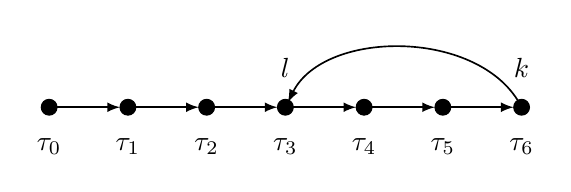
\begin{tikzpicture}
    \foreach \x in {0,1,2,3,4,5,6} 
    \draw[fill] (\x,5.5) circle (0.1);
    \foreach \x in {0,1,2,3,4,5} 
    \draw[-latex,semithick] (\x,5.5) -- +(0.9,0);
    \draw[-latex,shorten >=2,semithick] (6,5.5) .. controls (5.5,6.5) and (3.5,6.5) .. (3,5.5);
    \foreach \x in {0,1,2,3,4,5,6}
    \node at (\x,5) {$\tau_{\x}$};
    % \node at (-0.5,5) {$t=$};
    \node at (6,6) {$k$};
    \node at (3,6) {$l$};
  \end{tikzpicture}
  \caption{Some funny picture}
  \label{fig:def:prelim:ltl:kl-loop}
\end{figure}

\subsection{Referenzen}

Referenzen werden in einer Datenbank abgelegt (hier unter {\ttfamily 99--references.bib}) und dann im Text wie folgt referenziert \cite{Bringhurst1993}. \textcite{Bringhurst1993} schrieb die "`Bibel der Typografie"'. 

\subsection{Abkürzungen}

Abkürzungen müssen in wissenschaftlichen Texten bei der ersten Verwendung definiert (erklärt). Dies wird hier durch den Befehl \verb+\ac+ erledigt. 

Beispiel: Der Begriff \ac{LTL} wurde soeben definiert und bei der weiteren Verwendung von \ac{LTL} wird nurnoch die Abkürzung ausgegeben. Die Definitionen liegen zentral in der Datei \verb+acronyms.tex+. 

\subsection{Aufzählungen und Aufzählungspunkte}
Nummerierte Aufzählungen:
\begin{enumerate}
	\item Foo
    	\begin{enumerate}
        	\item kann auch 
        	\item verschachtelt werden
        \end{enumerate}
	\item Bar
\end{enumerate}

Nicht nummerierte Aufzählungen:
\begin{itemize}
	\item One
	\item Two
	\item Three
\end{itemize}

\subsection{Tabellen}
Eine Tabelle wie jene in \autoref{tab:example} 
kann etwas einfacher mittels \url{http://www.tablesgenerator.com} erstellt werden. 

Hinweise:
\begin{itemize}
    \item Tabellen werden normalerweise oben beschriftet. 
    \item Aus typografischer Sicht sind vertikale Linien in Tabellen "`schlechter Stil"', die Spalten sollten aufgrund der Abstände erkennbar sein. 
\end{itemize}

\begin{table}
	\centering
	\caption{Beispiel für eine Tabelle}
	\label{tab:example}
	\begin{tabular}{llc}
	\toprule
	A & B & C\\
	\midrule
	1 & 2 & unknown\\
	x & y & z\\
	\bottomrule
	\end{tabular}
\end{table}

\subsection{ToDo-Notizen}

\begin{todobox}
ToDo: Diplomarbeit mit sinnvollen Inhalten füllen. 
\end{todobox}

\subsection{Quellcode-Listings}

Listings möglichst nicht als Screenshot einbinden (verpixeln, nicht änderbar, kein Seitenumbruch möglich,~\ldots), siehe \autoref{lst:java}. 

Weitere Hinweise siehe \zB \url{https://www.overleaf.com/learn/latex/Algorithms#Listings_package}. 

\begin{lstlisting}[style=text,language=Java,label=lst:java,caption={Java Code Example}]
@FacesConverter(forClass = Fraction.class)
public class FractionConverter implements Converter {
    @Override
    public Object getAsObject(FacesContext context,
            UIComponent component, String value) {
        try {
            // split at the first slash
            String[] parts = value.split("/");
            return new Fraction(Integer.valueOf(parts[0]),
                    Integer.valueOf(parts[1]));
        } catch (NumberFormatException | IndexOutOfBoundsException e) {
            throw new ConverterException(
                    new FacesMessage(FacesMessage.SEVERITY_ERROR,
                            "Not a valid fraction!", null));
        }
    }
    @Override
    public String getAsString(FacesContext context,
            UIComponent component, Object value) {
        return ((Fraction) value).toString();
    }

}
\end{lstlisting}

% weitere individuelle teile

\chapter{Zusammenfassung und Ausblick}

Zusammenfassung der Ergebnisse (Schlussfolgerungen, eventuell Ergebnisvergleich mit anderen Arbeiten)

Persönliches Fazit, Reflexionsergebnisse zur Teamarbeit

Eventuell Empfehlung konkreter Maßnahmen




% \input{template/example-style-chapter}

\appendix

\addpart*{Anhänge}

\LDinsertbibliography

\listoffigures

\listoftables

\chapter{List of Abbreviations}
\begin{acronym}[MOMS]
\acro{ASP}{Answer Set Programming}
\acro{ATMS}{Assumption-based Truth Maintenance System}
\acro{BCP}{Boolean Constraint Propagation}
\acro{BDD}{Binary Decision Diagram}
\acro{BMC}{Bounded Model Checking}
\acro{CDCL}{Conflict-Driven Clause Learning}
\acro{CNF}{Conjunctive Normal Form}
\acro{CSP}{Constraint Satisfaction Problem}
\acro{CTL}{Computation Tree Logic}
\acro{DAG}{Directed Acyclic Graph}
\acro{DNF}{Disjunctive Normal Form}
\acro{DP}{Davis Putnam}
\acro{EDA}{Electronic Design Automation}
\acro{GDE}{General Diagnostic Engine}
\acro{GUI}{Graphical User Interface}
\acro{LTL}{Linear Temporal Logic}
\acro{MBD}{Model-Based Diagnosis}
\acro{MCS}{Minimal Correction Subset}
\acro{MHS}{Minimal Hitting Set}
\acro{MOMS}{Maximum Occurence in clauses of Minimum Size}
\acro{MUC}{Minimal Unsatisfiable Core}
\acro{OEMS}{Odd-Even Mergesort}
\acro{PSL}{Property Specification Language}
\acro{RAM}{Random Access Memory}
\acro{RSS}{Resident Set Size}
\acro{RTL}{Register Transfer Level}
\acro{SAT}{Satisfiability}
\acro{SDE}{Switching Diagnostic Engine}
\acro{SERE}{Sequential Extended Regular Expression}
\acro{SFM}{Strong Fault Model}
\acro{SMT}{Satisfiability Modulo Theories}
\acro{SOA}{Service Oriented Architecture}
\acro{SSD}{Solid State Drive}
\acro{SVA}{SystemVerilog Assertions}
\acro{TP}{Theorem Prover}
\acro{UC}{Unsatisfiable Core}
\acro{WFM}{Weak Fault Model}
\end{acronym}



\chapter{Verfasserverzeichnis}

Gibt es neben den individuellen Teilen, noch zusätzlich eine umfangreiche gemeinsame Vorstudie, dann ist ein Verfasserverzeichnis sinnvoll.



\chapter{Begleitprotokolle}

\section{Schüler 1}

\section{Schüler 2}

\section{Schüler 3}


\input{93--stundennachweise}

Weitere Anhänge nach Bedarf:

\begin{itemize}
\item Benutzerhandbuch
\item Administrationshandbuch
\item Sprintberichte
\item  Besprechungsprotokolle
\end{itemize}


\end{document}

